\documentclass[12pt,
border=1pt]{standalone}
\usepackage{pgfplots}
\usepackage{amsmath}
\usepackage{amssymb}

\pgfplotsset{compat=newest,
	width=6cm, height=5cm,
	xtick pos=left, ytick pos=left
	%            scaled x ticks=real:1e-6,
}
% Kernel 2 FP64
\begin{document}
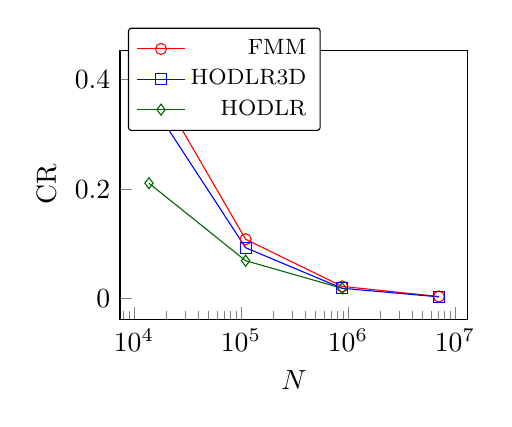
\begin{tikzpicture}
	\begin{axis}[xlabel={$N$},
	ylabel={CR},
%		legend pos=south east,
		legend style={
                at={(0.3,0.7)},
               anchor=south,
               legend columns=1,
               cells={anchor=east},
               font=\footnotesize,
               rounded corners=1pt,
               },
		xmode = log,
	   % ymode = log,
	   % xmin = 1e3,
	   % xmax = 1e6,
	   % ymin = 1e-10,
	   % ymax = 1e-0,
	   % xtick={1e-10, 1e-8, 1e-6,  1e-4,  1e-2},
	   % ytick={1e-8, 1e-6,  1e-4,  1e-2, 1e-0}
		]
		%Bebendrof
		\addplot[
		color=red,
		mark=o,
		] coordinates {
		(13824,0.412638)
(110592,0.108597)
(884736,0.022574)
(7077888,0.004101)
		};
		%Vaishnavi
		\addplot[
		color=blue,
		mark=square,
		] coordinates {
(13824,0.363393)
(110592,0.093165)
(884736,0.019094)
(7077888,0.003444)
		};
		%Zhao
		\addplot[
		color=black!60!green,
		mark=diamond,
		] coordinates {
(13824,0.210825)
(110592,0.069450)
(884736,0.019125)
		};
		\legend{FMM, HODLR3D, HODLR}
	\end{axis}
\end{tikzpicture}
\end{document}